\documentclass[a4paper, 12pt]{article}
\usepackage[T2A]{fontenc}
\usepackage[utf8]{inputenc}
\usepackage[english,russian]{babel}
\usepackage{amsmath, amsfonts, amssymb, amsthm, mathtools, misccorr, indentfirst, multirow}
\usepackage{wrapfig}
\title{Лабораторная работа 4.6.2\\ТУННЕЛИРОВАНИЕ
НА СВЕРХВЫСОКИХ ЧАСТОТАХ}
\date{\today}
\author{Александр Нехаев, гр 654}
\begin{document}
	\maketitle
	\pagenumbering{gobble}
	\newpage
	\tableofcontents
	\pagenumbering{arabic}
	\newpage
	\section{Введение}
	\paragraph{Цель работы:}изучение явления проникновения электромагнитного поля во вторую среду при полном внутреннем отражении (туннелирование) и использование этого явления для создания интерференционных схем в СВЧ-диапазоне.\par
	\paragraph{В работе используются:}генератор СВЧ-колебаний; излучающая и приемная рупорные антенны; детектор; две фторопластовые призмы; металлические зеркала; микроамперметр; плоскопа- раллельная пластина из фторопласта.\par
	\paragraph{Теоретические основы:}
	Плоские электромагнитные волны, распространяющиеся в однородной изотропной среде, описываются выражением
	\begin{equation}
		\boldsymbol{E}=\boldsymbol{a}e^{-i\left(\omega t-\boldsymbol{kr}\right)}=\boldsymbol{a}e^{i\left(k_xx+k_yy+k_zz\right)}e^{-i\omega t}=\boldsymbol{A}\left(x,y,z\right)e^{-\omega t}.
		\label{eq:1}
	\end{equation}
	В данном выражении:\par
	\begin{enumerate}
		\item $\boldsymbol{a}$ — амплитуда вектора напряженности электрического поля
		\item $\boldsymbol{E,r}$ — радиус-вектор точки наблюдения
		\item $\omega$ — круговая частота волны
		\item $\boldsymbol{k}$ — волновой вектор
	\end{enumerate}
	Направление вектора $\boldsymbol{k}$ совпадает с направлением распространения волны, а модуль этого вектора:
	\begin{equation*}
		k=\frac{2\pi}{\lambda}=\frac{\omega}{v}
	\end{equation*}
	где $v$ – фазовая скорость распространения волн в рассматриваемой среде. Комплексна запись (\ref{eq:1}) позволяет вместо тригонометрических функций использовать более удобную экспоненциальную форму
	\begin{equation}
		\boldsymbol{A}\left(x,y,z\right)=\boldsymbol{a}e^{i\left(k_xx+k_yy+k_zz\right)}
	\end{equation}
	Эта векторная величина называется \textit{комплексной амплитудой волны}.\par
	Значения $k_x$, $k_y$ и $k_z$ могут быть как действительными (однородная плоская волна), так и мнимыми (неоднородные волны).\par
	Рассмотрим волну вида (\ref{eq:1}) с мнимым значением $k_z=\pm i\boldsymbol{\varkappa}$:
	\begin{equation}
		\boldsymbol{E}=\boldsymbol{a}^{\pm\boldsymbol{\varkappa}}e^{i\left(k_xx+k_yy\right)}e^{-i\omega t}
		\label{eq:3}
	\end{equation}
	Выражение (\ref{eq:3}) описывает бегущую волну, амплитуда которой экспоненциально затухает (или нарастает) по оси $Z$. Неоднородные волны возникают и вблизи границы раздела двух сред при полном внутреннем отражении света.\par
	На границе раздела двух сред происходит преломление и отражение световых волн. Формулы для интенсивности, направления распространения, поляризации отраженных и преломленных волн, могут быть получены из граничных условий для векторов $\boldsymbol{E}$, $\boldsymbol{D}$, $\boldsymbol{H}$ и $\boldsymbol{B}$:
	\begin{equation}
		E_{1\tau}=E_{2\tau},\quad D_{1n}=D_{2n}, H_{1\tau}=H_{2\tau}, B_{1n}=B_{2n}
		\label{eq:4}
	\end{equation}
	$\tau$ — тангенциальные, $n$ — нормальные составляющие.\\
	\begin{wrapfigure}{1}{4cm}
		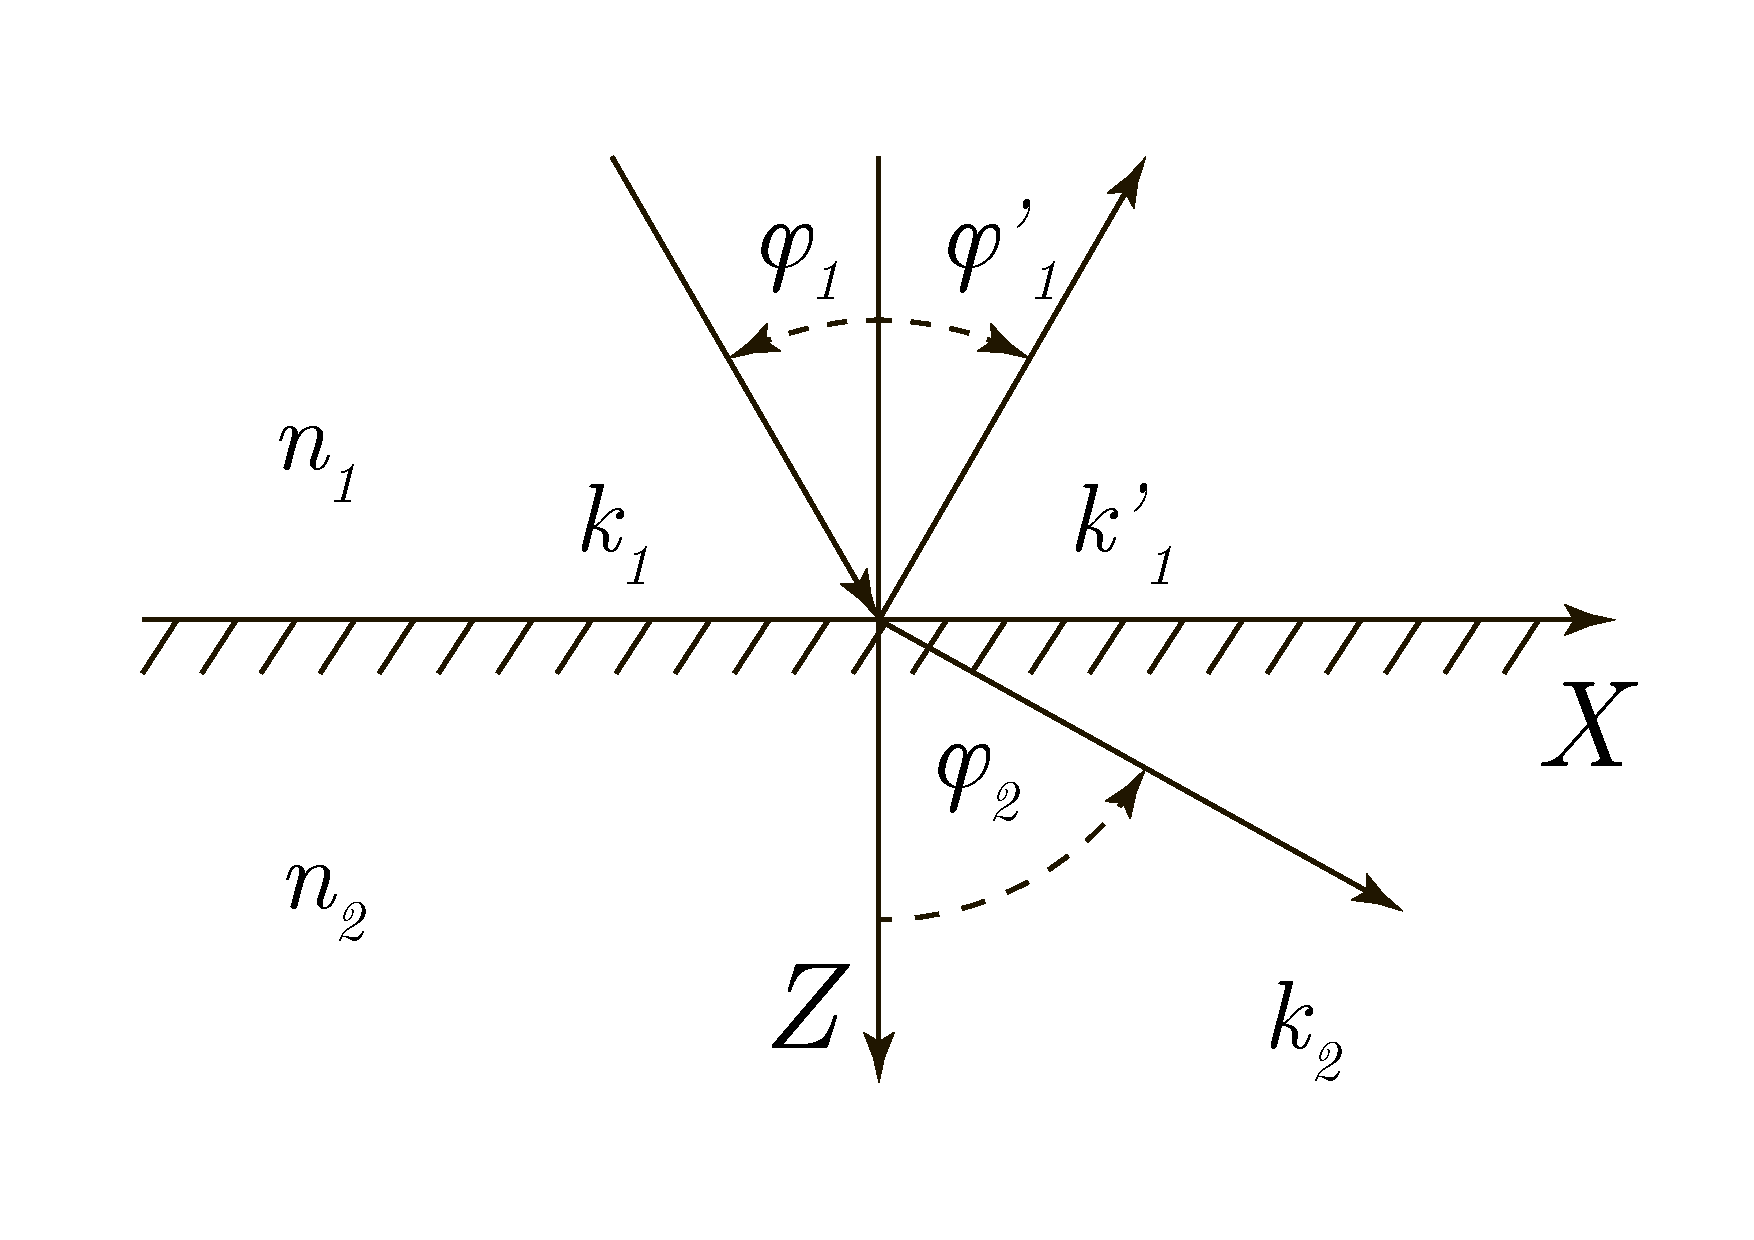
\includegraphics[scale=0.2]{Graph1.pdf}
		\caption{Преломление волн на границе раздела двух сред}	
		\label{fig:pic1}
	\end{wrapfigure}
	1 — первая среда, 2 — вторая среда. В электромагнитной волне элекрическая и магнитная составляющие связаны между собой, из четырех соотношений в (\ref{eq:4}) независимыми остаются только два. Используем условия для тангенциальных компонент полей.\par
	Выберем координатную систему так, как это изображено на рис. \ref{fig:pic1}. Ось $Z$ совпадает с нормалью к поверхности раздела сред. Ось $X$ лежит в плоскости падения светового луча. $\boldsymbol{E}_1$, $\boldsymbol{E}_1'$ и $\boldsymbol{E}_2$ — электрические поля в падающей, отраженной и преломленной волнах соответственно:
	\begin{equation}
		\boldsymbol{E}_1=\boldsymbol{a}_1e^{i\left(k_1x\sin\varphi_1 + k_1z\cos \varphi_1 \right)}e^{-i\omega_1 t};
		\label{eq:5}
	\end{equation}
	\begin{equation}
		\boldsymbol{E}_1'=\boldsymbol{a}_1'e^{i\left(k_1'x\sin\varphi_1' + k_1'z\cos \varphi_1' \right)}e^{-i\omega_1' t};
		\label{eq:6}
	\end{equation}
	\begin{equation}
		\boldsymbol{E}_2=\boldsymbol{a}_2e^{i\left(k_2x\sin\varphi_1 + k_2z\cos \varphi_1 \right)}e^{-i\omega_2 t};
		\label{eq:7}
	\end{equation}
	Здесь
	\begin{enumerate}
		\item $\varphi_1$ — угол падения
		\item $\varphi_1'$ — угол отражения
		\item $\varphi_2$ — угол преломления
	\end{enumerate}
	\par
	На границе раздела (при $z=0$) должны выполняться граничные условия (\ref{eq:5}, \ref{eq:6}, \ref{eq:7}). Первое из них дает: $E_{1\tau}+E_{1\tau}'=E_{2\tau}$, или
	\begin{equation*}
		a_1e^{ik_1x\sin\varphi_1}e^{-i\omega_1 t}+a_1'e^{ik_1'x\sin\varphi_1'}e^{-i\omega_1' t}=a_2e^{ik_2x\sin\varphi_2}e^{-i\omega_2 t}
	\end{equation*}
	Это равенство выполняется при любых значениях $t$ и $x$. Поэтому:
	\begin{equation}
		\omega_1=\omega_1'=\omega_2
		\label{eq:8}
	\end{equation}
	\begin{equation}
		k_1\sin\varphi_1=k_1'\sin\varphi_1'=k_{2x}
		\label{eq:9}
	\end{equation}
	Равенство (\ref{eq:8}) показывает, что частоты отраженной и преломленной волн равны по частоте падающей волны.\par
	Падающая и преломленная волна распространяются в одной среде, значит
	\begin{equation}
		k_1'=k_1
	\end{equation}
	Учитывая (\ref{eq:9}):
	\begin{equation}
		\sin\varphi_1=\sin\varphi_1'
	\end{equation}
	то есть угол падения равен углу отражения.\par
	Пусть волна во второй среде однородна, тогда $k_2=k_2\sin\varphi_2$ и, следовательно, на основании (\ref{eq:9}):
	\begin{equation}
		\frac{\sin\varphi_1}{\sin\varphi_2}=\frac{k_2}{k_1}=\frac{v_1}{v_2}=\frac{n_2}{n_1}=\frac{1}{n}
		\label{eq:12}
	\end{equation}
	$n_1$ и $n_2$ — показатели преломления первой и второй сред соответственно. Получили закон преломления световых лучей. Накладывая граничные условия (например $H_{1\tau}=H_{2\tau}$, на (\ref{eq:5}-\ref{eq:7}) можно получить соотношение между амплитудами $a_1$, $a_1'$ и $a_2$ всех трёх волн (формулы Френеля).\par
	Легко показать, что при падении света на границу раздела со стороны оптически более плотной среды ($n_1>n_2$) формула (\ref{eq:12}) теряет смысл, когда угол падения $\varphi_1$ превышает некоторое критическое значение $\varphi_\text{пр}$, которое носит название \textit{предельного угла полного внутреннего отражения:}
	\begin{equation}
		\sin\varphi_\text{пр}=\frac{n_2}{n_1}=\frac{k_2}{k_1}
	\end{equation}
	\par
	При $\varphi_1>\varphi_\text{пр}$ в формуле (\ref{eq:12}) $\sin\varphi_2$ оказывается больше единицы. Это означает, что наше предположение об однородности волны во второй среде в случае полного внутреннего отражения оказывается несправедливым.\par
	Попытаемся теперь удовлетворить граничным условиям и вытекающему из них соотношению (\ref{eq:9}), предположив:, что волна во второй среде является неоднородной. При $\varphi_1>\varphi_\text{пр}$ получим
	\begin{equation}
		k_1\sin\varphi_1>k_1\sin\varphi_\text{пр}=k_1\frac{k_2}{k_1}=k_2
	\end{equation}
	При сравнении с (\ref{eq:9}) найдем
	\begin{equation}
		k_{2x}>k_2
	\end{equation}
	Но
	\begin{equation}
		k_2^2=k_{2x}^2+k_{2z}^2
	\end{equation}
	Разрешая уравнение относительно $k_{2z}$, найдем
	\begin{equation}
		k_{2z}=\pm\sqrt{k_2^2-k_{2x}^2}=\pm i \sqrt{k_{2x}^2-k_2^2}=\pm i\sqrt{k_1^2\sin^2\varphi_1-k_2^2}
	\end{equation}
	$k_{2z}$ называется мнимой величиной. Волна во второй среде неоднородна и описывается выражением виде (\ref{eq:3}), где $k_y=k_{2y}=0$, $k_x=k_{2x}=k_1\sin\varphi_1$, а величина $\varkappa$:
	\begin{equation}
		\varkappa=\sqrt{k_1^2\sin^2\varphi_1-k_2^2}
	\end{equation}
	Экспоненциальную функцию, описывающую затухание волны с удалением от поверхности раздела, удобно записать в виде $\exp\left(-z/2\Lambda\right)$. Тогда интенсивность волны изменяется с расстоянием по закону
	\begin{equation}
		I\sim e^{-z/\Lambda}
		\label{eq:19}
	\end{equation}
	Длина затухания $\Lambda$ равна
	\begin{equation}
		\Lambda=\frac{1}{2\sqrt{k_1^2\sin^2\varphi_1-k_2^2}}=\frac{1}{2k_2\sqrt{n^2\sin^2\varphi_1-1}}=\frac{\lambda_2}{4\pi\sqrt{n^2\sin^2\varphi_1-1}}
		\label{eq:20}
	\end{equation}
	Эти две формулы позволяют количественно исследовать затухание электромагнитных колебаний во второй среде.\par
	Отметим, что при полном внутреннем отражении сдвиг фаз между отраженной и падающей волнами не равен нулю и зависит от поляризации падающей волны. Вследствие этого изменяется поляризация света: плоскополяризованная волна после отражения оказывается поляризованной по эллипсу.\par
	\paragraph{Формулы Френеля}
	\begin{equation}
		R+T=1
	\end{equation}
	\begin{enumerate}
		\item $T\rightarrow 1$ и $R\rightarrow 0$ при ширине, стремящейся к нулю.
		\item $R\rightarrow 1$ и $T\rightarrow 0$ при увеличении ширины прослойки
	\end{enumerate}
	Проникновение электромагнитных волн в менее плотную среду при полном внутреннем отражении — явление той же природы, что и проникновение частиц в область, где их полная энергия оказывается меньше потенциальной энергии. Это явление изучается в квантовой физике и носит название \textit{туннельного эффекта}. Классическим примером является $\alpha$-распад радиоактивных ядер. По аналогии, прохождение электромагнитных волн через узкий зазор при углах падения, превосходящих угол полного внутреннего отражения, часто называют \textit{туннелированием}.
	\section{Экспериментальная установка}
	\begin{figure}[h]
		\centering
		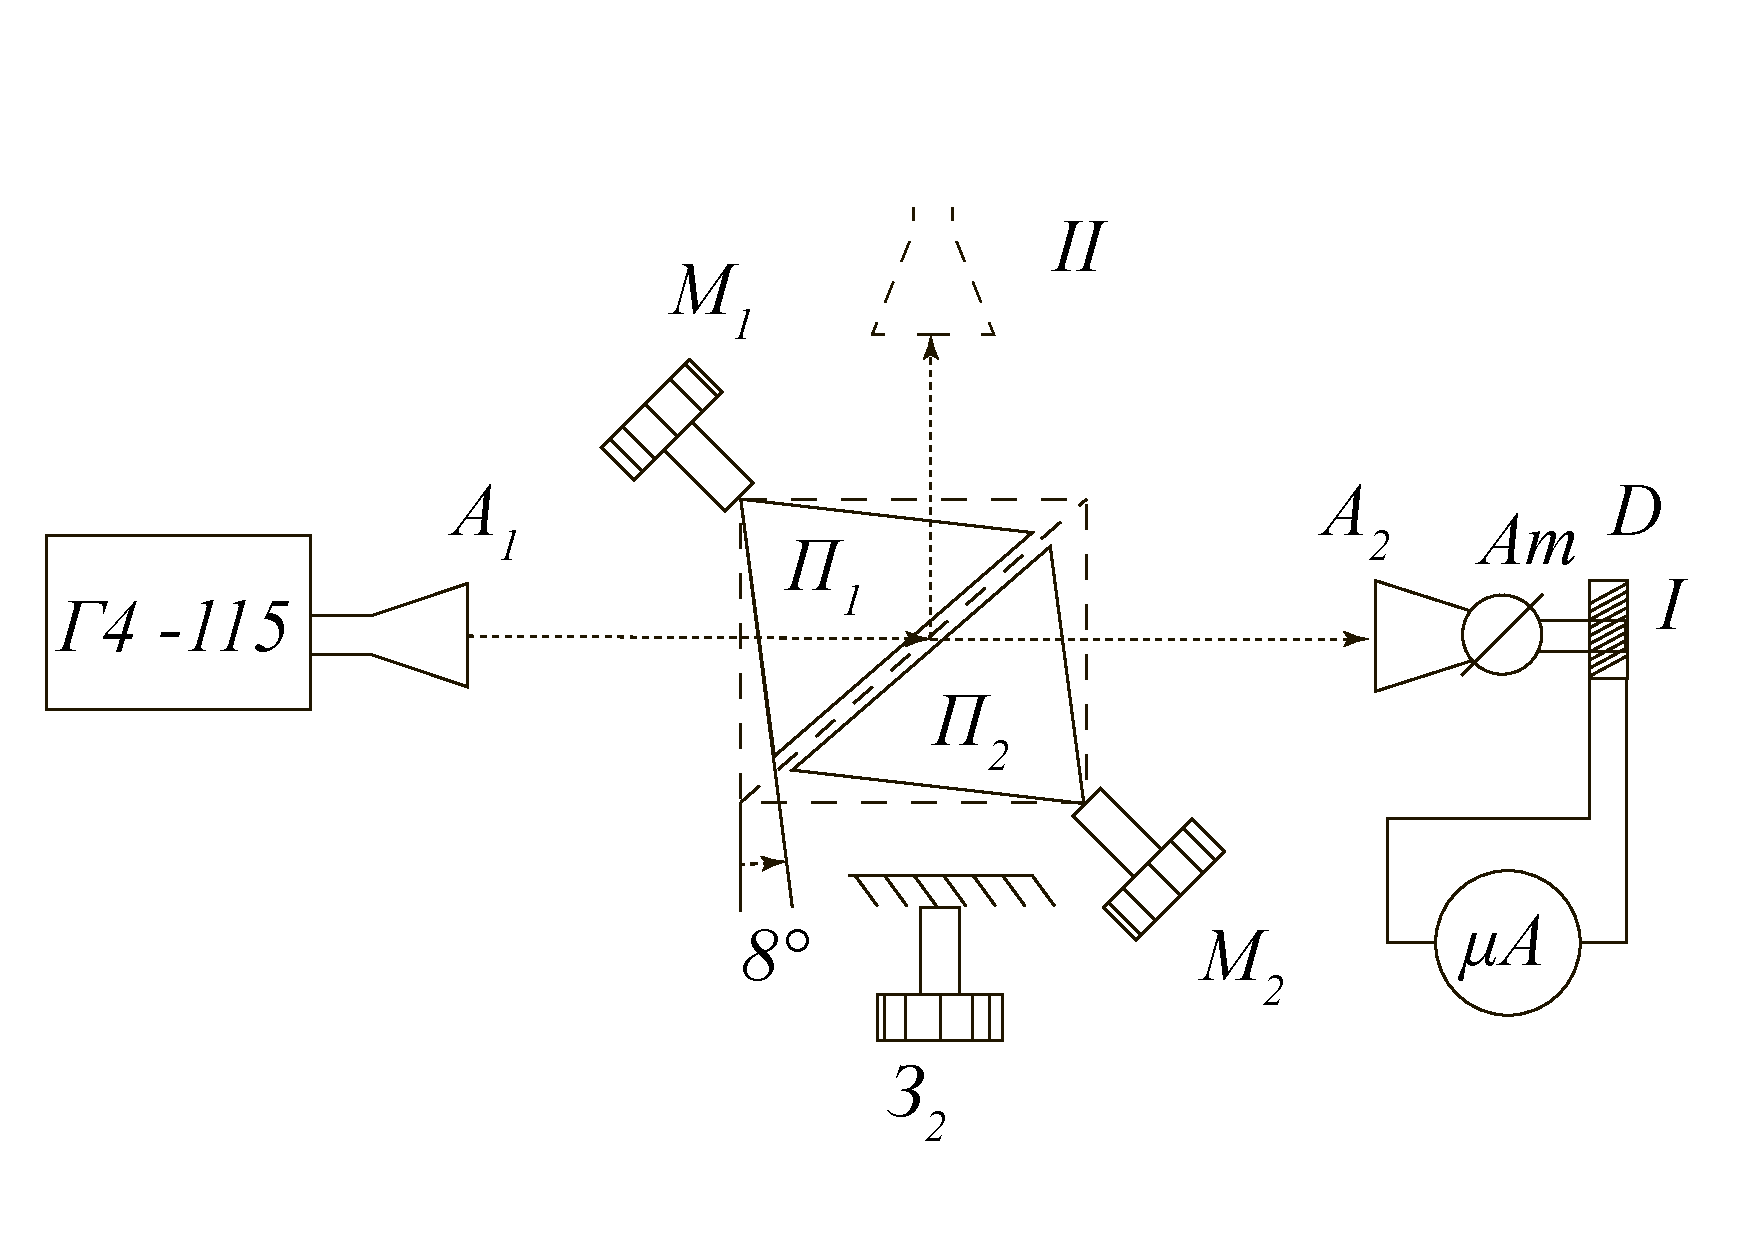
\includegraphics[scale=0.4]{Facility.pdf}
		\caption{Схема установки для исследования явления туннелировния СВЧ-радиоволн}
		\label{fig:experimental}
	\end{figure}
	Туннелирование СВЧ-радиоволн через тонкий воздушный зазор переменной толщины изучается по схеме на рис. \ref{fig:experimental}. На пути радиоволн устанавливаются две призмы $\Pi_1$ и $\Pi_2$, изготовленные из фторпласта — диэлектрика с малыми потерями на высоких радиочастотах.\par
	Источником радиоволн служит СВЧ-генератор Г4-115, работающий в непрерывном режиме. Основным элементом генерачтора является специальная лампа — клистрон, генерирующая СВЧ-колебания. От клистрона к рупорной антенне $A_1$ энергия СВЧ-колебаний передается по прямоугольному волноводу. Клистрон возбуждает в волноводе линейно поляризованную электромагнитную волну, которая с помощью рупорной антенны излучается в пространство. Электрический вектор волны, бегущей вдоль волновода и излучаемый антенной, перпендикулярен широкой стенке волновода. Вторая рупорная антенна $A_2$ служит приёмником волн. Попадая в антенну $A_2$, электромагнитная волна распространяется далее в волноводе. Детектор $D$, расположенный в волноводе, подсоединяется к микроамперметру. Ток детектора пропорционален интенсивности принимаемого антенной электромагнитного излучения. Аттенюатор $A_\text{т}$ ослабляет сигнал.\par
	В положении I антенна $A_2$ принимает сигнал, прошедший воздушный промежуток, в положении II — сигнал, отраженной от воздушного промежутка.\par
	\begin{wrapfigure}{2}{5cm}
		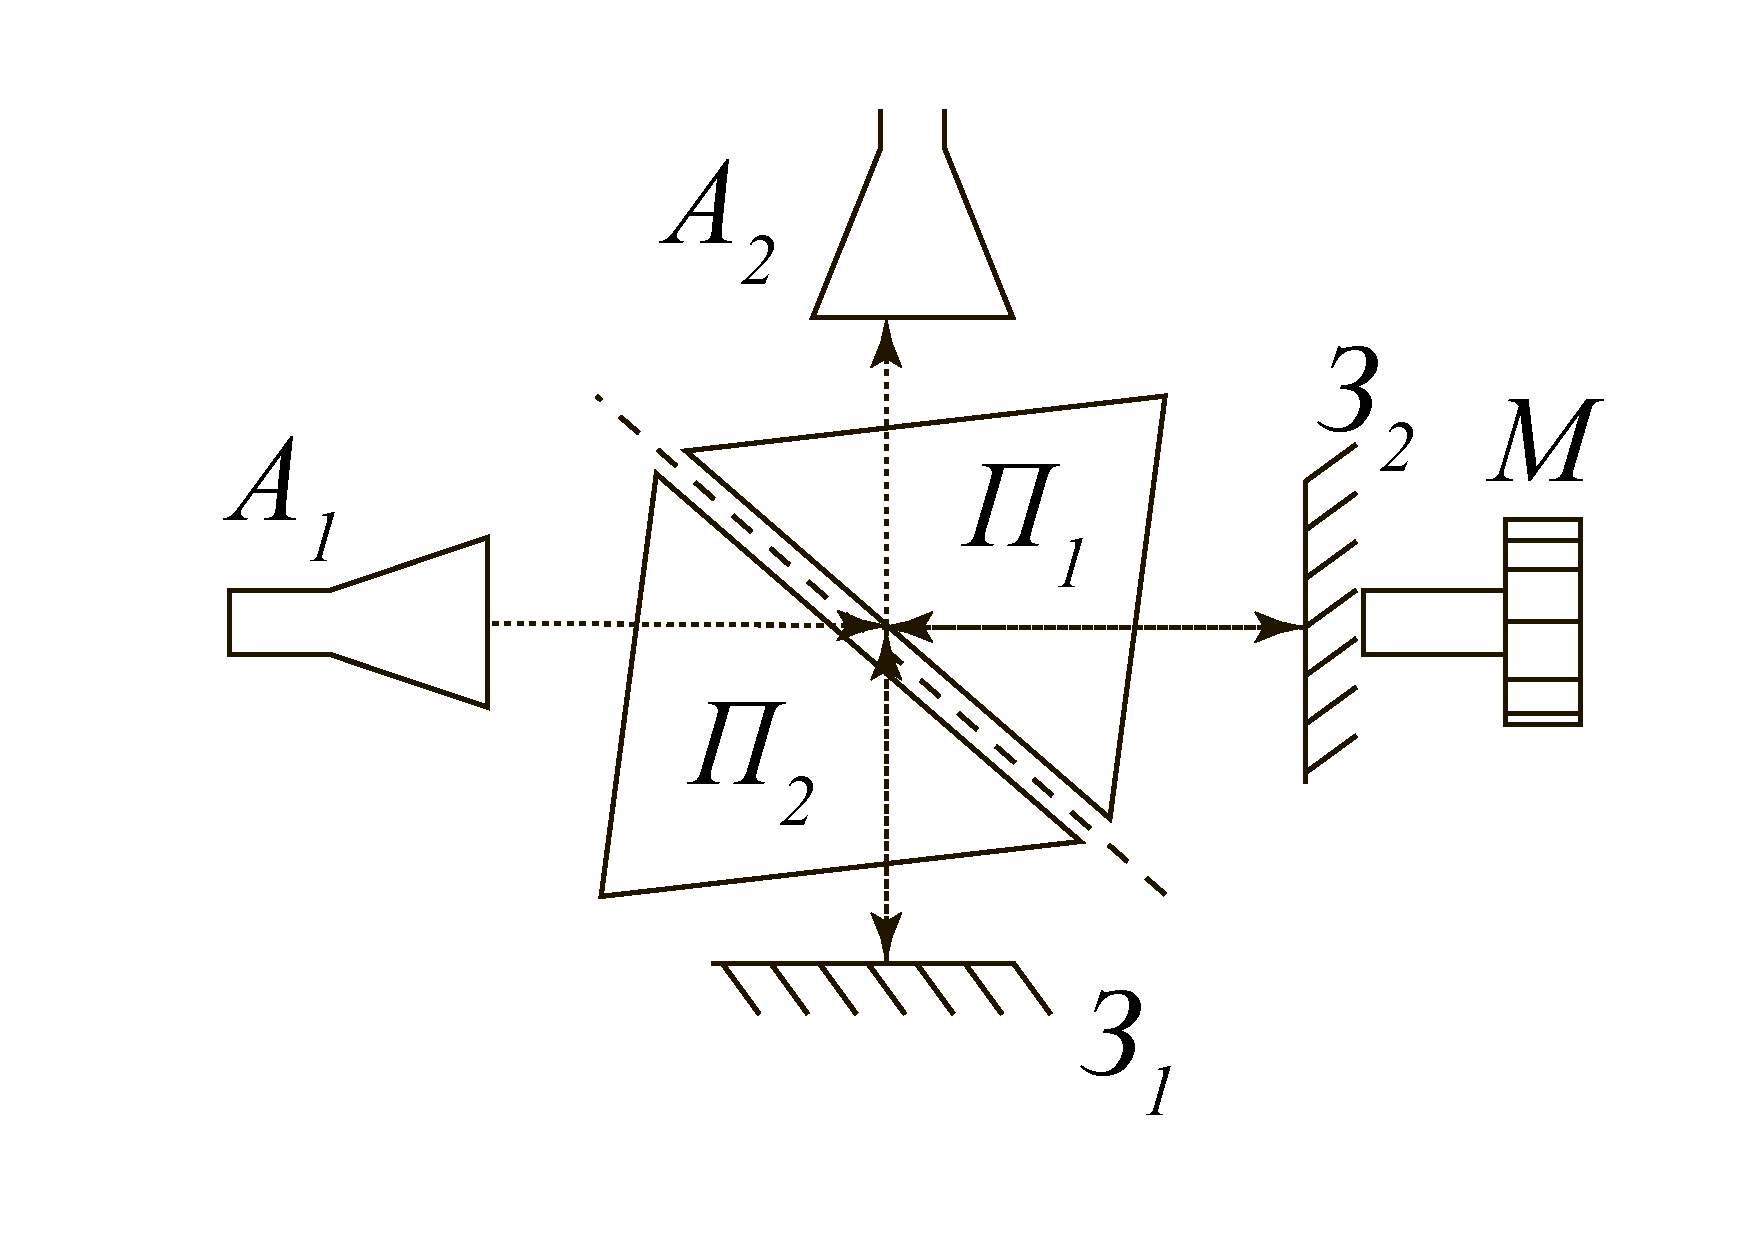
\includegraphics[scale=0.18]{Michelson.pdf}
		\caption{Схема, моделирующая интерферометр Майкельсона}
		\label{fig:Michelson}
	\end{wrapfigure}

	Установка позволяет смоделировать интерферометр Майкельсона (рис. \ref{fig:Michelson}). В качестве делителя используется воздушный зазор между диагональными гранями призм; зеркало $\text{З}_1$ установлено неподвижно, зеркало $\text{З}_2$ может перемещаться с помощью микрометрического винта $M$.\par
	Для измерения показателя преломления материала призм интерференционным методом перед неподвижным зеркалом устанавливается пластинка из фторпласта известной толщины $d$. В этом плече интерферометра возникает приращение длины оптического пути $\Delta=2d\left(n-1\right)$. Можно скомпенсировать это приращение, передвинув зеркало на необходимое расстояние $x_0$. Показатель преломления определяется из условия
	\begin{equation}
		x_0=d\left(n-1\right).
		\label{eq:22}
	\end{equation}
	Для толстых пластин, когда $\Delta>\lambda$, необходимо учесть изменение порядка интерференции. Это можно сделать, зная приближённое значение показателя преломления фторпласта $\left(n\simeq 1,5\right)$.
	\section{Ход работы}
	\subsection{Подготовока приборов к работе}
	\begin{enumerate}
		\item Настроим генератор, руководствуясь техническим описанием, расположенном на установке.
		\item Установим столик с призмами так, чтобы воздушный зазор был ориентирован под углом $45^\circ$ к падающему лучу. Вращением винта правого микрометра ($M_2$) уберем воздушный промежуток.
		\item Расположим приёмную антенну на одной прямой с передатчиком. Снимем металлическое зеркало, стоящее на пути луча. Методом последовательных приближений добьемся максимального отклика микроамперметра.
		\item Настроим генератор на максимальную выходную мощность клистрона.
		\item Добъемся загорания красной лампочки и определим рабочую частоту клистрона по шкале. Рассчитаем соответствующую длину волны.
		$\lambda=8.58$ мм.
	\end{enumerate}
	\subsection{Зависимости коэффициентов отражения и прохождения волны от величины зазора}
	\begin{enumerate}
		\item Снимем зависимость интенсивности прошедшей волны от величины зазора $l$, используя правый микрометр.
		\begin{table}[h]
			\centering
				\begin{tabular}{|c|c|c|c|}
				\hline
  				$l$, мм (без вычета)& $l$, мм & $I$, мкА & $I$, мкА (нормированная)\\
  				\hline
  				7 & 2 & 82 & 0,82\\
				7,5 & 2,5 & 62 & 0,62\\
				8 & 3 & 47 & 0,47\\
				8,5 & 3,5 & 37 & 0,37\\
				9 & 4 & 29 & 0,29\\
				9,5 & 4,5 & 22 & 0,22\\
				10 & 5 & 17 & 0,17\\
				10,5 & 5,5 & 14 & 0,14\\
				\hline
			\end{tabular}
		\end{table}
		\item Переставим приёмник для измерения отражённого сигнала. Снимем зависимость интенсивности отражёнvй волны от величины зазора.
		\begin{table}[h]
			\centering
			\begin{tabular}{|c|c|c|c|}
				\hline
				$l$, мм & $l$, мм & $I$, мкА & $I$, мкА (нормированная)\\
				\hline
				5,5 & 0,5 & 0 & 0\\
				6 & 1 & 9 & 0,09\\
				6,5 & 1,5 & 27 & 0,27\\
				7 & 2 & 47 & 0,47\\
				7,5 & 2,5 & 65 & 0,65\\
				8 & 3 & 78 & 0,78\\
				8,5 & 3,5 & 88 & 0,88\\
				9 & 4 & 93 & 0,93\\
				9,5 & 4,5 & 95 & 0,95\\
				10 & 5 & 100 & 1\\
				10,5	 & 5,5 & 98 & 0,98\\
				\hline
			\end{tabular}
		\end{table}
		\item Установим такую величину зазора, при которой ток равен половине максимального. Убедимся в том, что $T\simeq R\simeq 0,5$.
		\item Построим на одном листе графики зависимости коэффициентов $T$ и $R$ от величины зазора $l$, пронормировав токи на величину $I_{\max}$. Проверим выполнения соотношения $T+R=1$.
		\begin{figure}[h]
			\centering
			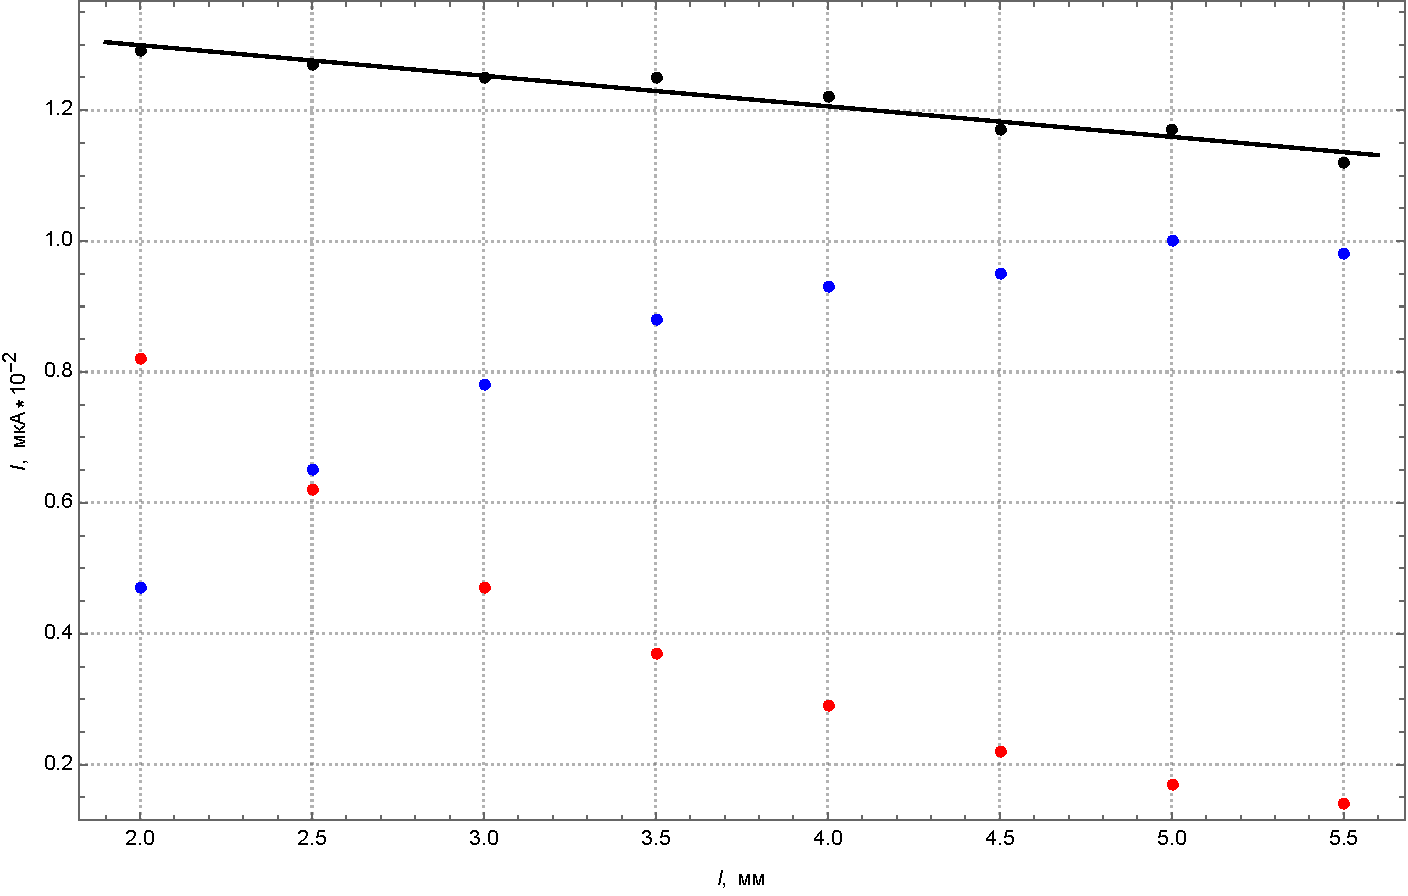
\includegraphics[scale=0.57]{Graphic.pdf}
			\caption{Зависимость $I(l)$}
		\end{figure}
		\item Построим график $\log{T}=f\left(z\right)$, где $z$ — показания микрометра. Проверим, лежит ли полученные точки на одной прямой согласно требованию формулы (\ref{eq:19}) По наклону прямой рассчитаем длину затухания $\Lambda$, а затем по формуле (\ref{eq:20}) — величину $n\sin\varphi_1$ ($n$ — показатель преломления материала призм, $\varphi_1$ — угол падения волны на воздушный промежуток, $\lambda_2$ — длина СВЧ-волны в воздухе). Рассчитаем величину $n$; при этом в условиях нашего опыта можно не учитывать, что входная плоскость призмы $\Pi_1$ наклонена на угол $\varphi=8^\circ$ по отношению к фронту падающей волны.
		\newpage
		\begin{figure}[h]
			\centering
			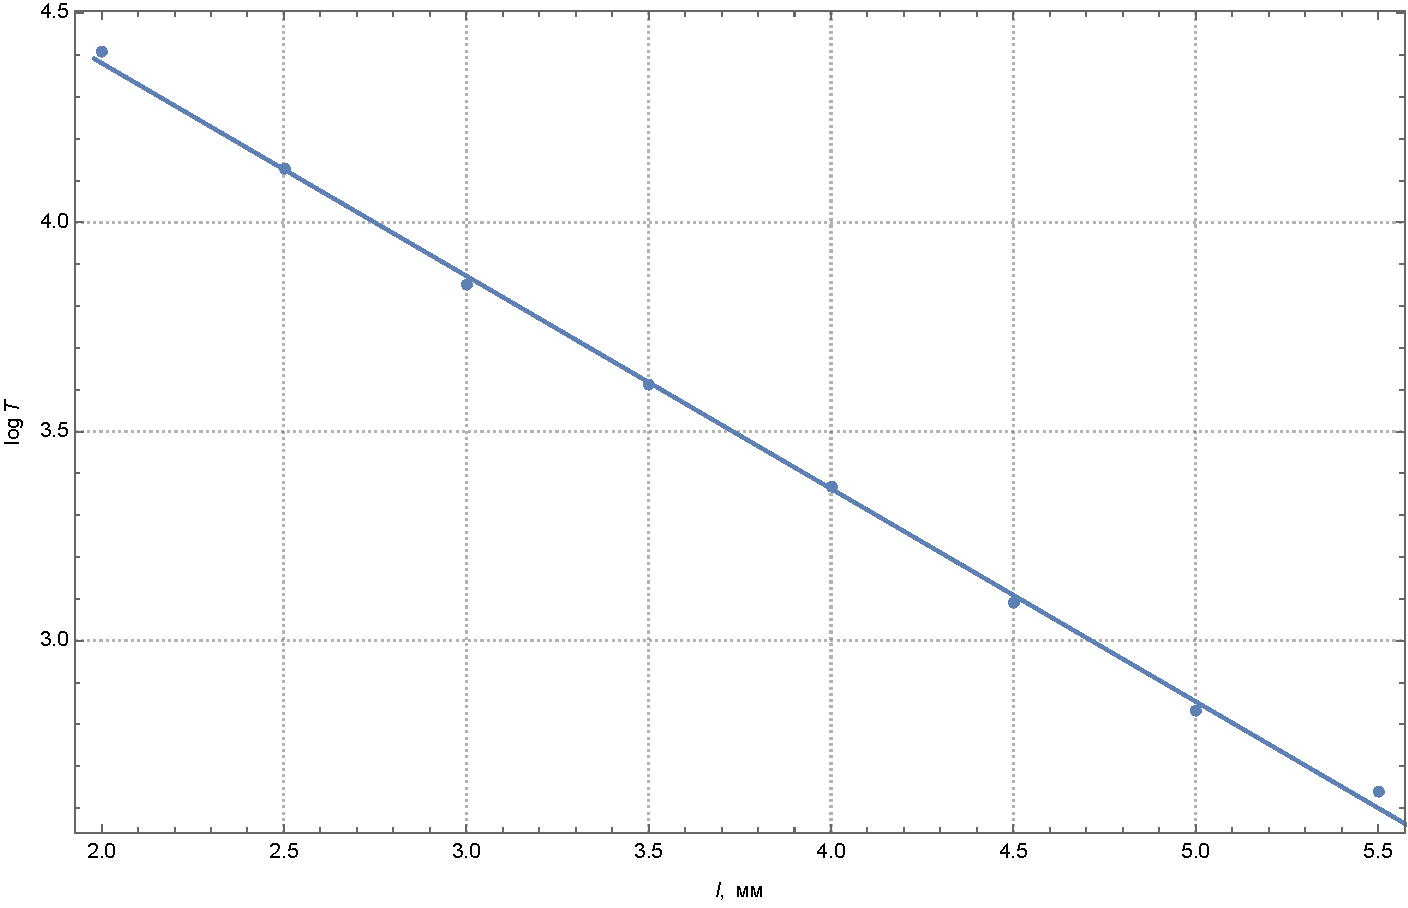
\includegraphics[scale=0.57]{Graphic2.pdf}
			\caption{Зависимость $\log T(l)$}
		\end{figure}
		Полученная методом наименьших квадратов формула линии аппроксимации:
		\begin{equation}
			y=5.39821 - 0.508671 x
		\end{equation}
		То есть $\Lambda=0.508671$.\par
		Формула для расчета $n\sin\varphi_1$:
		\begin{equation}
			n=\frac{\sqrt{16\pi\Lambda^2+\lambda_2^2}}{4\pi\Lambda\sin\varphi_1}=1.67383
		\end{equation}
	\end{enumerate}
	\subsection{Интерферометр Майкельсона}
	\begin{enumerate}
		\item Соберем схему интерферометра Майкельсона (рис. \ref{fig:Michelson}), используя в качестве делителя воздушный зазор между призмами. Оптимальный размер зазора соответствует равенству $T\simeq R\simeq 0,5$. Установим на место неподвижное металлическое зеркало.
		\item Снимем зависимость тока от координаты $x$ подвижного зеркала. По графику $I=f\left(x\right)$ определим экспериментальное значение длины волны СВЧ-излучения.\par
			Обычно максимумы размыты, поэтому определение длины волны будет более точным, если взять координаты, соответствующие максимальным производным $dI/dx$. Сравним экспериментальную длину волны с величиной, рассчитанной по частоте.
			\begin{table}[h]
				\centering
				\begin{tabular}{|c|c|c|}
					\hline
					$l$, мм (без вычета)& $x$, мм & $I$, мкА\\
					\hline
					5 & 0 & 45\\
					5,05 &	0,05 & 50\\
					5,1 & 0,1 & 52\\
					5,15 & 0,15 & 55\\
					5,2 & 0,2 & 59\\
					5,25 & 0,25 & 62\\
					5,3 & 0,3 & 66\\
					5,35 & 0,35 & 70\\
					\hline
				\end{tabular}
			\end{table}
			\begin{figure}[h]
				\centering
				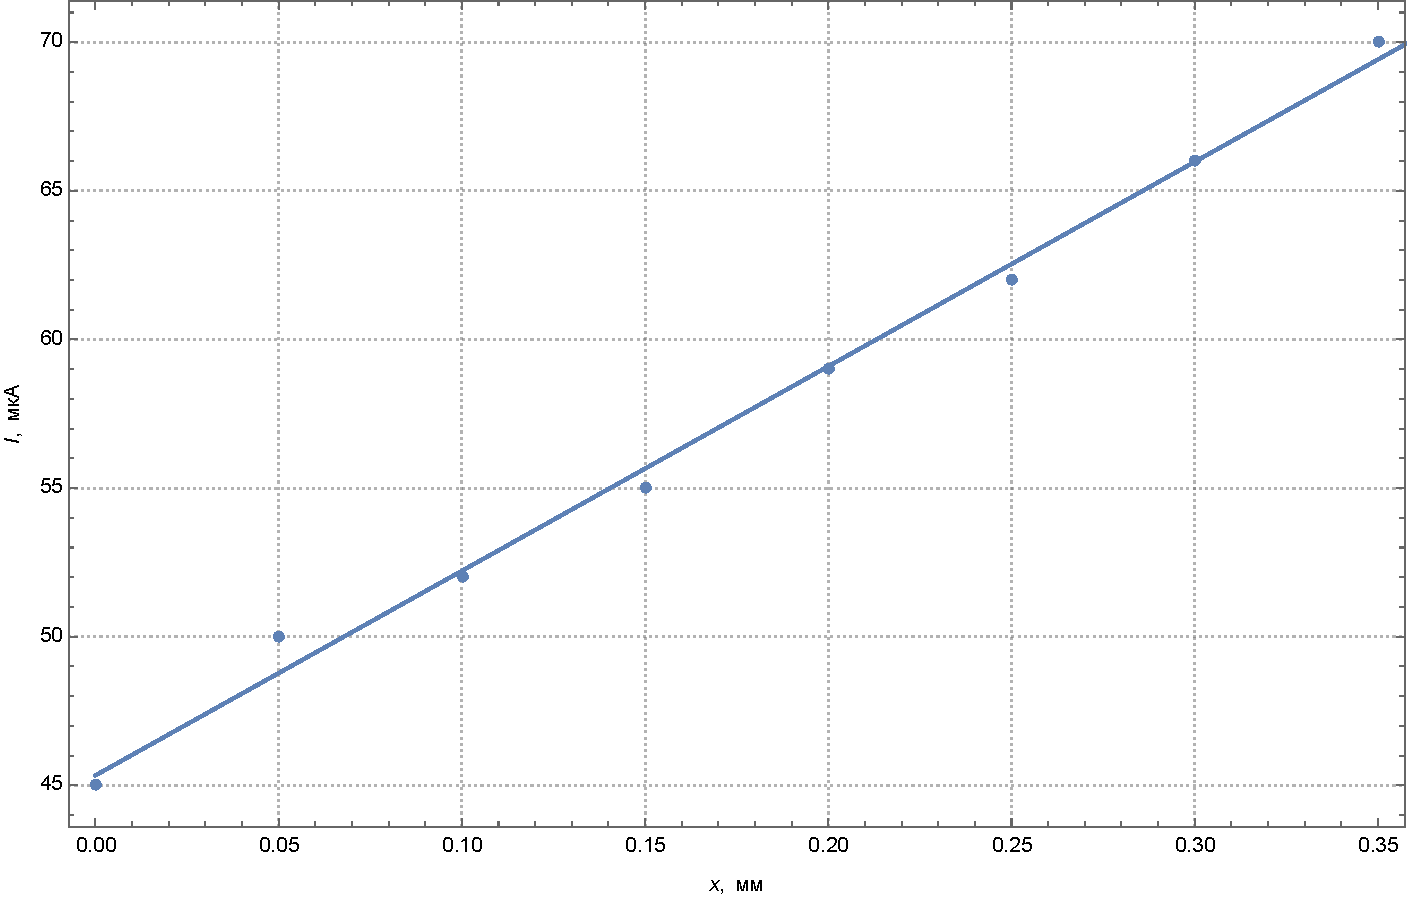
\includegraphics[scale=0.55]{Graphic3.pdf}
			\end{figure}
		\item Для измерения показателя преломления фторопласта интерференционным методом настроим интерферометр на максимальную интенсивность и поместим пластину известной толщины $d$ перед неподвижным зеркалом. Скомпенсируем возникшее увеличение оптической длины пути, передвинув (удалив от призм) подвижное зеркало на необходимое расстояние $x_0$. Рассчитаем показатель преломления фторопласта по формуле (\ref{eq:22}).\par
		$d=0.62 \text{ мм}$, $x_0=0.35\text{ мм}$
		\begin{equation}
			x_0=d(n-1)\Rightarrow n=\frac{x_0}{d}+1=1.5645
		\end{equation}
		\item Сравним результаты измерения $n$ интерференционным методом и методом туннелирования\par
		\begin{equation}
			n_\text{интер}=1.5645\quad n_\text{туннел}=1.67383
		\end{equation}
	\end{enumerate}
	\section{Вывод}
		Мы изучили явление полного отражения при проникновении электромагнитного поля в во вторую среду те туннелирование и использование данного метода для создания СВЧ волн. Сравнили полученные показатели преломления при туннелировании и интерференции и получили маленькое расхождение.
 \end{document}